\documentclass[fleqn,10pt]{wlscirep}
\usepackage[utf8]{inputenc}
\usepackage[T1]{fontenc}
\title{Beyond metastability}

\author[1,*]{Kalel Luiz Rossi}
\author[2]{Robson budnizisk}
% \author[1,2,+]{Christine Author}
% \author[2,+]{Derek Author}
% \affil[1]{Affiliation, department, city, postcode, country}
% \affil[2]{Affiliation, department, city, postcode, country}

\affil[*]{corresponding.author@email.example}
% \affil[+]{these authors contributed equally to this work}


\keywords{Metastability}

\begin{abstract}
abstract
\end{abstract}
\begin{document}

\flushbottom
\maketitle
% * <john.hammersley@gmail.com> 2015-02-09T12:07:31.197Z:
%
%  Click the title above to edit the author information and abstract
%
\thispagestyle{empty}

% \noindent Please note: Abbreviations should be introduced at the first mention in the main text – no abbreviations lists. Suggested structure of main text (not enforced) is provided below.

\section*{Introduction}

\begin{itemize}
    \item 
\end{itemize}


\section*{Results}
% Up to three levels of \textbf{subheading} are permitted. Subheadings should not be numbered.


\subsection*{Network Synchronization}
% \subsubsection*{Third-level section}

\begin{figure}[ht]
\centering
% 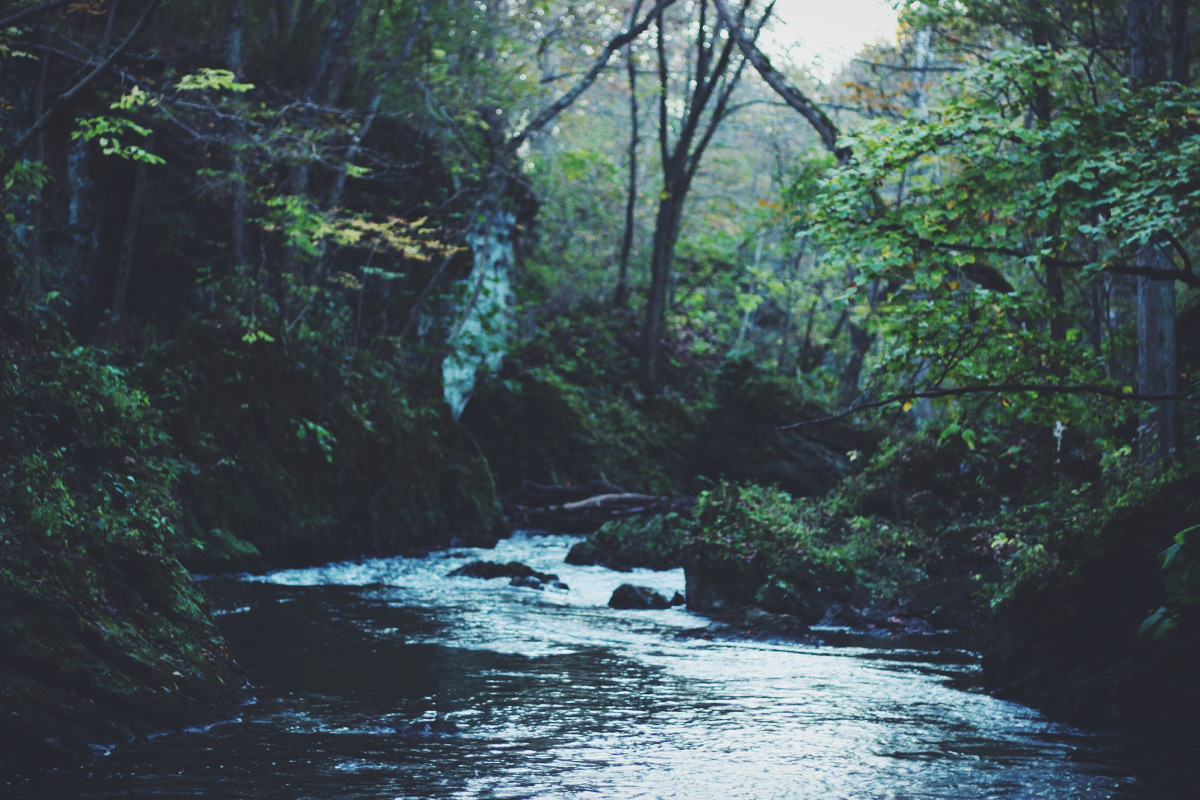
\includegraphics[width=\linewidth]{stream}
\caption{Legend (350 words max). Example legend text.}
\label{fig:stream}
\end{figure}

\subsection*{Metastability I - global }
std(R)

\begin{figure}[ht]
\centering
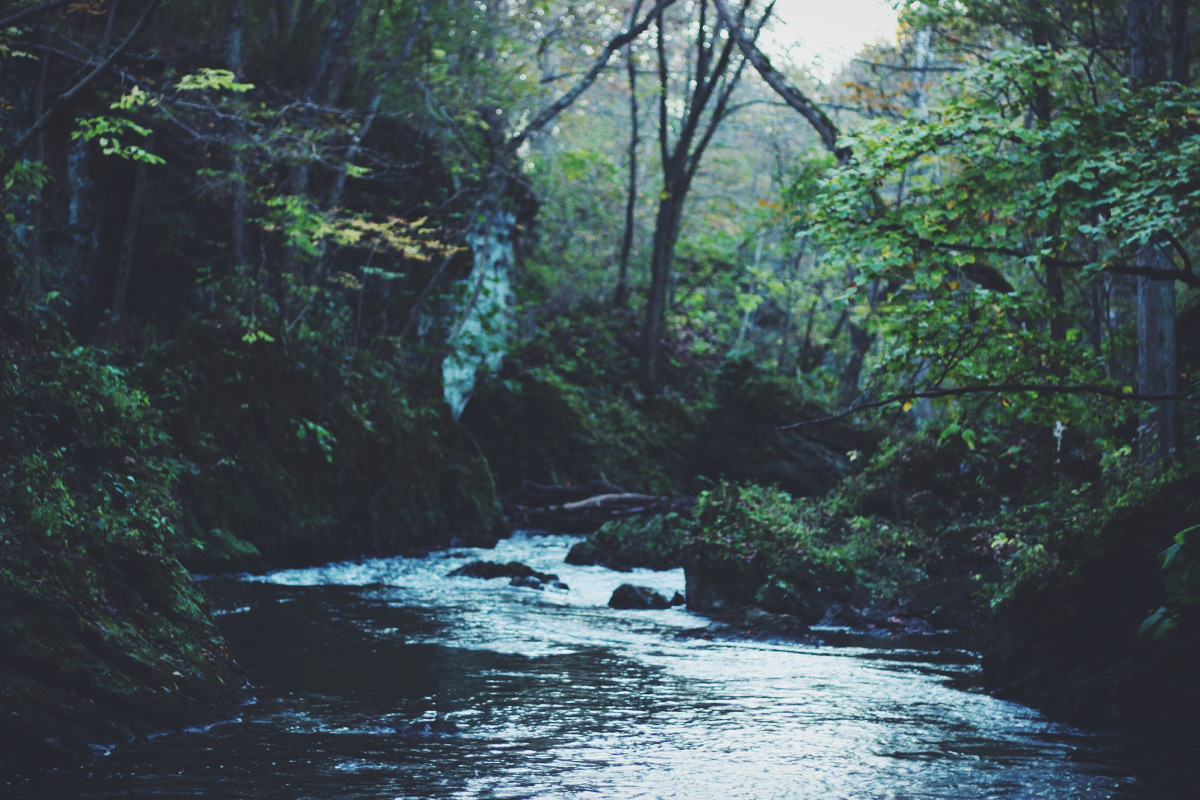
\includegraphics[width=\linewidth]{stream}
\caption{Legend (350 words max). Example legend text.}
\label{fig:stream}
\end{figure}


\subsection*{Metastability  II - local }
Rij

\begin{figure}[ht]
\centering
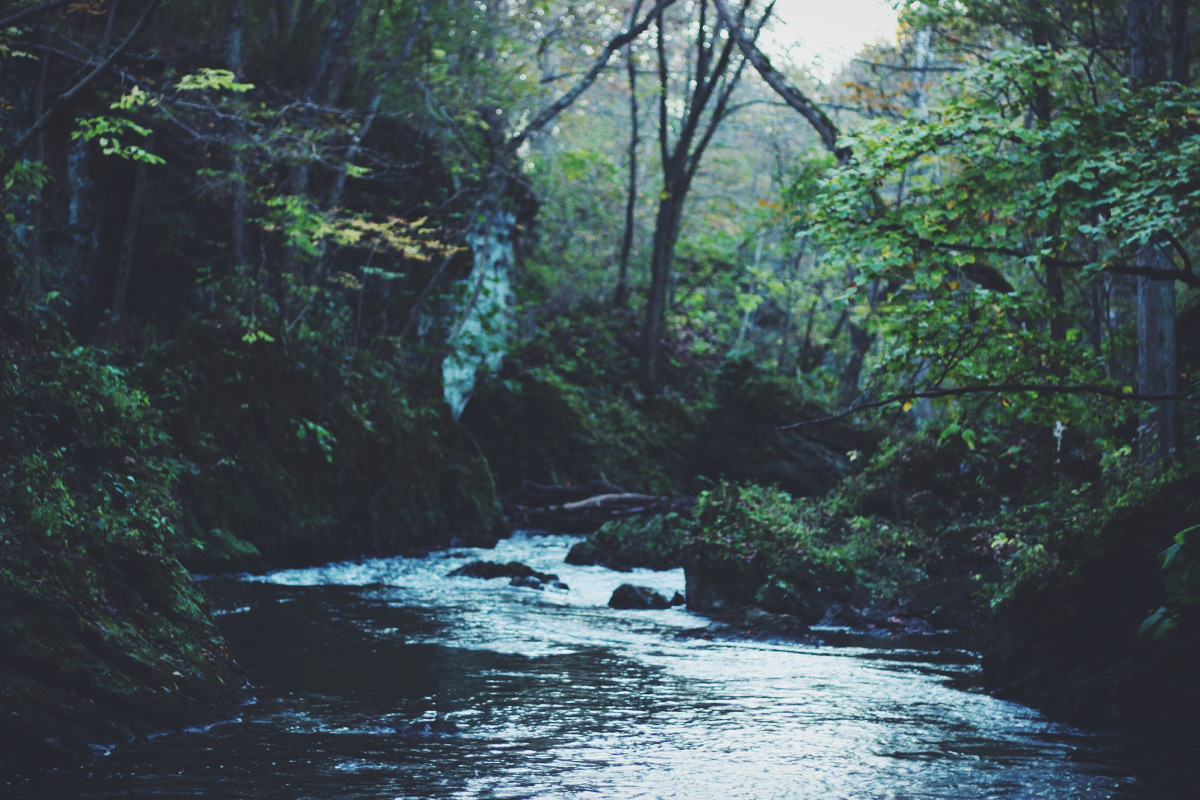
\includegraphics[width=\linewidth]{stream}
\caption{Legend (350 words max). Example legend text.}
\label{fig:stream}
\end{figure}


\subsection*{Metastability III - cluster }

\begin{figure}[ht]
\centering
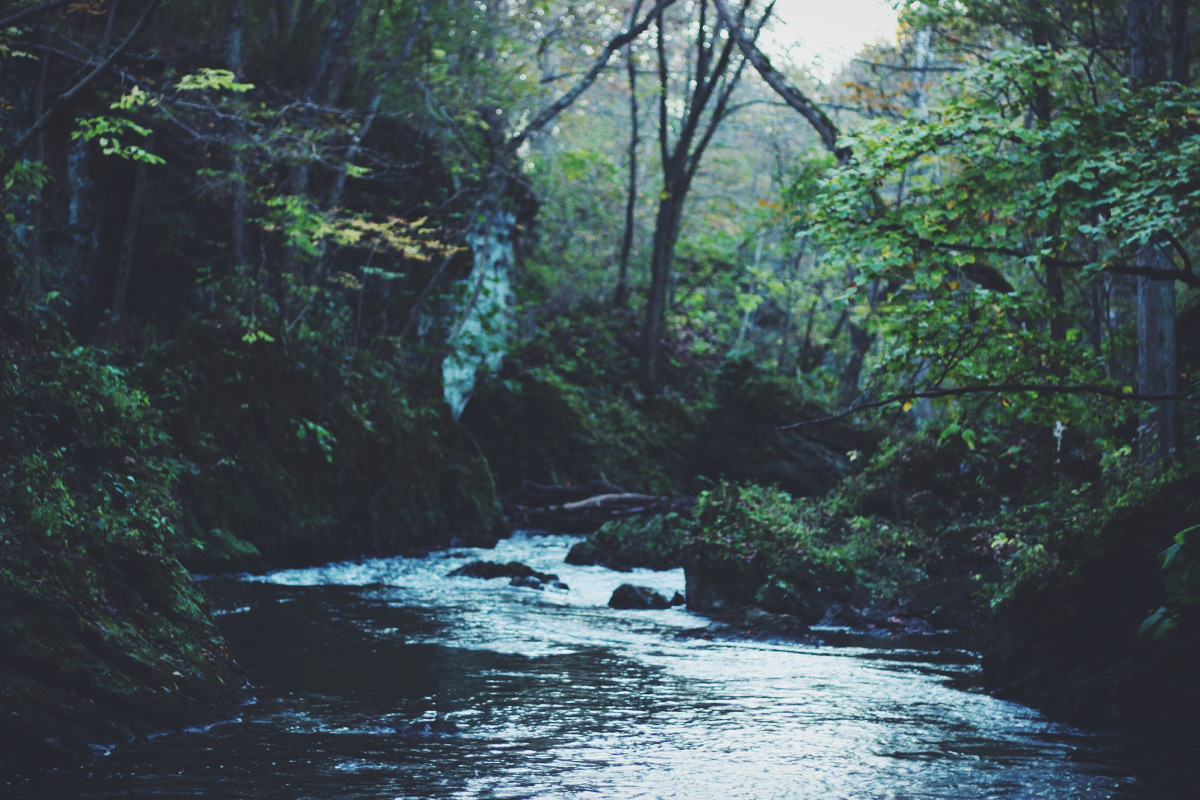
\includegraphics[width=\linewidth]{stream}
\caption{Legend (350 words max). Example legend text.}
\label{fig:stream}
\end{figure}
\subsection*{Intermittency}


 Figuras
 \begin{enumerate}
    \item neural dynamics
     \item <R>, std(R), std(Rij), M (cluster) 
     \item Series temporais R(t), Rij(t)
     \item Analise cluster: Tamanho do GC por epsilon, decaimento do GC por numero de interseçoes 
     \item Intermitencia
 \end{enumerate}

opçao 2: deixar a figura geral opr ultimo


\section*{Discussion}
% The Discussion should be succinct and must not contain subheadings.











\section*{Methods}
\begin{equation}
    R_{jk}(t) = \frac{1}{2}\left| e^{i \phi_j(t)} + e^{i \phi_k(t)} \right|,
\end{equation}


\bibliography{sample}



\section*{Acknowledgements (not compulsory)}


\section*{Author contributions statement}

Must include all authors, identified by initials, for example:
A.A. conceived the experiment(s),  A.A. and B.A. conducted the experiment(s), C.A. and D.A. analysed the results.  All authors reviewed the manuscript. 

\section*{Additional information}

To include, in this order: \textbf{Accession codes} (where applicable); \textbf{Competing interests} (mandatory statement). 

The corresponding author is responsible for submitting a \href{http://www.nature.com/srep/policies/index.html#competing}{competing interests statement} on behalf of all authors of the paper. This statement must be included in the submitted article file.

% \begin{figure}[ht]
% \centering
% 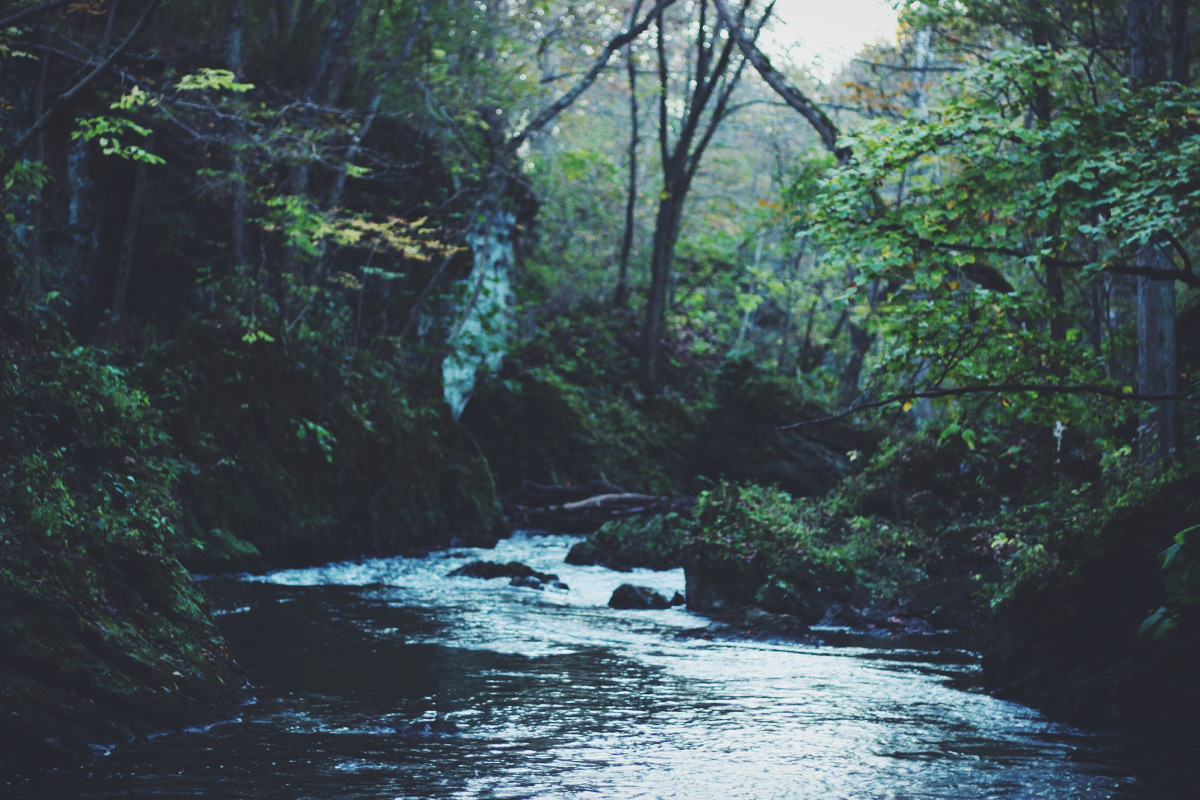
\includegraphics[width=\linewidth]{stream}
% \caption{Legend (350 words max). Example legend text.}
% \label{fig:stream}
% \end{figure}

% \begin{table}[ht]
% \centering
% \begin{tabular}{|l|l|l|}
% \hline
% Condition & n & p \\
% \hline
% A & 5 & 0.1 \\
% \hline
% B & 10 & 0.01 \\
% \hline
% \end{tabular}
% \caption{\label{tab:example}Legend (350 words max). Example legend text.}
% \end{table}

% Figures and tables can be referenced in LaTeX using the ref command, e.g. Figure \ref{fig:stream} and Table \ref{tab:example}.

\end{document}